\begin{wideslide}[bm=,toc=]{Mutual induction for automata}
\begin{figure}[h]
\centering
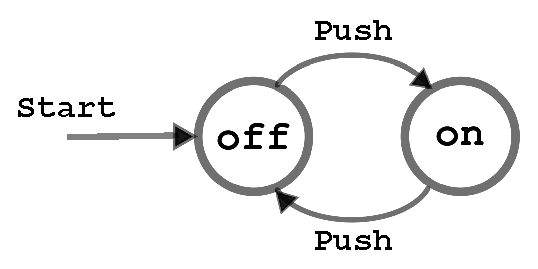
\includegraphics[width=2.5in, height=.75in,keepaspectratio=true]{switch.eps}
\label{2sp}
\end{figure}

{\bf Theorem}. For the on-off automaton, we prove the following: 
\begin{itemize}
\item $S_1(n)$: The automaton is in state {\em off\/} after $n$ pushes iff $n$ is even.

\item $S_2(n)$: The automaton is in state {\em on\/} after $n$ pushes iff $n$ is odd.
\end{itemize}
{\bf Proof}.  By {\em weak\/} mutual induction on the number of pushes, $n$. 

\end{wideslide}

\begin{wideslide}[bm=,toc=]{Inductive Hypothesis}

Since the two statements given are biconditional, we will split them into four
implications. Here, $n$ represents the number of pushes that have been applied to
the automaton:
\begin{tabbing}
{\bf Sx(n)}XX \=  (only-if) \= \kill
{\bf $S_1(n)$}  \>
           \bf{if:} \> 
          $n$ is even $\implies$ the automaton is {\em off\/}.   \\[2ex]
               \>
     \bf{only-if:}\> 
          The automaton is {\em off\/} $\implies$ $n$ is even.   \\[4ex]
{\bf $S_2(n)$} \>
          \bf{if:} \> 
        $n$ is odd $\implies$ the automaton is {\em on\/}. \\[2ex]
               \>
     \bf{only-if:} \> 
        The automaton is {\em on\/} $\implies$ $n$ is odd. \\[2ex]
\end{tabbing}

\end{wideslide}

\begin{wideslide}[bm=,toc=]{Basis}

\begin{tabbing}
{\bf Sx(n)}XX \=  (only-if) \= \kill
{\bf $S_1(0)$}  \>
           \bf{if:} \> 
           $0$ is even, so we must show the automaton is off after $0$ pushes.  \\
      \>\> Since the start state is off, this is the case.  \\[2ex]
      \>
     \bf{only-if:}\> 
          The automaton is {\em off\/} after $0$ pushes, so we must show that $0$ is\\ 
      \>\>   even. This is true by definition.   \\[4ex]
{\bf $S_2(0)$} \>
          \bf{if:} \> 
          Must prove: ``$0$ is odd $\implies$ the automaton is {\em
                   on\/}.'' This is\\
     \>\> vacuously true.  \\[2ex]
     \>
     \bf{only-if:} \> 
       Must prove: ``The automaton is {\em on\/} after $0$ pushes 
                   $\implies$ $0$ is odd.'' \\
     \>\> Again, the antecedent is false, so the implication holds.\\[2ex]
\end{tabbing}


\end{wideslide}

\begin{wideslide}[bm=,toc=]{Inductive Step for $S_1$}
{\bf Show:} $S_1(n)$ and $S_2(n)$ imply $S_1(n + 1)$.\\
{\bf (Recall)} $S_1(n+1)$: The automaton is in state \emph{off} after $n + 1$
pushes iff $n+1$ is even.  
\begin{tabbing}
{\bf Sx(n + 1)}X \=  (only-if) \= \kill
{\bf $S_1(n + 1)$}  \>
           \bf{if:} \> 
           If $n + 1$ is even, $n$ is odd. By $S_2(n)$, the automaton is \\
      \>\> in the \emph{on} state after $n$ pushes. Applying one more push from \\
      \>\> this state switches from the \emph{on} state to the \emph{off} state (following\\
      \>\> the arc labeled ``Push''), so the automaton is in the \emph{off} state \\
      \>\> after $n + 1$ pushes. This proves $n + 1$ is even $\implies$ the  \\
      \>\> automaton is off.
           \\[2ex]
      \>
     \bf{only-if:}\> 
           If the automaton is in the \emph{off} state after $n + 1$ pushes, it must \\
      \>\> have been in the \emph{on} state after $n$ pushes. By $S_2(n)$, we have\\
      \>\> that $n$ must be odd, so $n+1$ is even. This proves that if the \\
      \>\> automaton is in the off state after $n + 1$ pushes, $n+1$ is even.
           \\[2ex]
\end{tabbing}


\end{wideslide}

\begin{wideslide}[bm=,toc=]{Inductive Step for $S_2$}
{\bf Show:} $S_1(n)$ and $S_2(n)$ imply $S_2(n + 1)$.\\
{\bf (Recall)} $S_2(n+1)$: The automaton is in state \emph{on} after $n + 1$
pushes iff $n+1$ is odd.  
\begin{tabbing}
{\bf Sx(n + 1)}X \=  (only-if) \= \kill
{\bf $S_1(n + 1)$}  \>
           \bf{if:} \> 
           If $n + 1$ is odd, $n$ is even. By $S_1(n)$, the automaton is \\
      \>\> in the \emph{off} state after $n$ pushes. Applying one more push from \\
      \>\> this state switches from the \emph{off} state to the \emph{on} state (following \\
      \>\> the arc labeled ``Push''), so the automaton is in the \emph{on} state \\
      \>\> after $n + 1$ pushes. This proves $n + 1$ is odd $\implies$ the \\
      \>\> automaton is on.
           \\[2ex]
      \>
     \bf{only-if:}\> 
           If the automaton is in the \emph{on} state after $n + 1$ pushes, it must \\
      \>\> have been in the \emph{off} state after $n$ pushes. By $S_1(n)$, we have\\
      \>\> that $n$ must be even, so $n+1$ is odd. This proves that if the \\
      \>\> automaton is in the on state after $n + 1$ pushes, $n+1$ is odd. 
           \\[2ex]
\end{tabbing}


\end{wideslide}



%{\bf Theorem}. If $t\in\id{RT}$ then $\id{\#edges}(t)$ = $\id{\#nodes}(t) - 1$.
%\vspace{1em}
%
%{\bf Proof}.  By {\em strong\/} mutual induction on derivation height. 
%We prove the following two statements:
%\vspace{1em}
%
%$S_1$: $l\in \id{RTL}\Rightarrow \id{\#edges}(l) = \id{\#nodes}(l) - |l|$.
%
%$S_2$: $t\in \id{RT}\Rightarrow \id{\#edges}(t) = \id{\#nodes}(t) - 1$.
%
%\vspace{2em}
%Note: $|l|$ stands for the length of list $l$, $\id{\#edges}(l)$ the number of edges in $l$
%and $\id{\#nodes}(l)$ the number of nodes in $l$.
%\end{wideslide}
%
%\begin{wideslide}[bm=,toc=]{Mutual induction}
%{\em Basis\/}: derivation height is zero.
%
%\vspace{1em}
%$S_1$: If derivation height is zero then $l\in\id{RTL}$ implies $l=\id{nil}$.
%Then $\id{\#edges}(\id{nil})=\id{\#nodes}(\id{nil}) - |\id{nil}| = 0$.
%
%\vspace{1em}
%$S_2$: Vacuously true since there's no derivation of height zero for $t\in\id{RT}$.
%
%\vspace{2em}
%{\em Inductive hypothesis\/}:  Suppose for all $k$ where $0\leq k\leq n$ and $n\geq 0$,
%$S_1$ holds if $l\in\id{RTL}$ has derivation height $k$ and
%$S_2$ holds if $t\in\id{RT}$ has derivation height $k$.
%\end{wideslide}
%
%\begin{wideslide}[bm=,toc=]{Mutual induction}
%{\em Inductive step}.
%We must show $S_1$ and $S_2$ for every derivation of height $n+1$ for $n\geq 0$.
%We begin with $S_2$.
%
%\vspace{1em}
%Suppose $t\in\id{RT}$ has derivation height $n+1$ where $n\geq 0$.
%Then the derivation must end with {\bf R2}. 
%Therefore $t$ has the form $\id{node}(x)$
%where $x\in\id{RTL}$.
%The derivation of $x\in\id{RTL}$ has height $n$.
%%So by induction and $S_1$, $\id{\#edges}(x)=\id{\#nodes}(x)$.
%Then
%\begin{displaymath}
%\begin{array}{lll}
%\id{\#nodes}(\id{node}(x)) & = & 1 + \id{\#nodes}(x) \\
%	& = & 1+\id{\#edges}(x) + |x|\;\;\;\rid{by induction and}\;S_1 \\
%	& = & 1+\id{\#edges}(\id{node}(x))
%\end{array}
%\end{displaymath}
%Ergo, $\id{\#edges}(\id{node}(x))=\id{\#nodes}(\id{node}(x))-1$.
%\end{wideslide}
%
%\begin{wideslide}[bm=,toc=]{Mutual induction}
%Now we show $S_1$.
%Suppose $l\in\id{RTL}$ has derivation height $n+1$ where $n\geq 0$.
%Then the derivation must end with {\bf R1}. 
%Therefore $l$ has the form $\id{cons}(x,y)$
%where $x\in\id{RT}$ and $y\in\id{RTL}$.
%Either the derivation of $x\in\id{RT}$ or $y\in\id{RTL}$ has height $n$ while the other 
%has height {\em at most\/} $n$.
%%By induction and $S_2$, $\id{\#edges}(x)=\id{\#nodes}(x)-1$.
%%Also by induction and $S_1$, $\id{\#edges}(y)=\id{\#nodes}(y)$.
%Then
%\begin{displaymath}
%\begin{array}{lll}
%\id{\#edges}(\id{cons}(x,y)) & = & \id{\#edges}(x) + \id{\#edges}(y) \\
%	& = & \id{\#nodes}(x) - 1 + \id{\#edges}(y) \\
% & & \>\>\>\>\>\>\rid{by induction and}\;S_2 \\
%	& = & \id{\#nodes}(x) - 1 + \id{\#nodes}(y) - |y| \\
% & & \>\>\>\>\>\>\rid{by induction and}\;S_1 \\
%	& = & \id{\#nodes}(\id{cons}(x,y)) - 1 - |y| \\
%	& = & \id{\#nodes}(\id{cons}(x,y)) - (1 + |y|) \\
%	& = & \id{\#nodes}(\id{cons}(x,y)) - |\id{cons}(x,y)|
%\end{array}
%\end{displaymath}
%%{\em quod erat demonstrandum (Q.E.D.)\/}
%\end{wideslide}
%
%
